\documentclass[11pt]{article}

% Packages
\usepackage{graphicx}   % for pictures
\usepackage{amsthm}     % for math
\usepackage{amsmath, mathtools}    %   more math
\usepackage{amsfonts}   %   more math
\usepackage{physics}    % more symbols
\usepackage{circuitikz} % for circuit diagrams
\usepackage{amssymb}    % math symbols
\usepackage{siunitx}    % units
\usepackage{mathrsfs}   % fancy text
\usepackage{color}      % colored letters for notes and reminders
\usepackage{float}      % for image location

%The amsthm package lets you format different types of mathematical ideas nicely. You use it by defining "\newtheorem"s as below:
\newtheorem{problem}{Problem}
\newtheorem{theorem}{Theorem}
\newtheorem*{proposition}{Proposition}
\newtheorem{lemma}[theorem]{Lemma}
\newtheorem{corollary}[theorem]{Corollary}
\theoremstyle{definition}
\newtheorem{defn}[theorem]{Definition}

% Magins

\setlength{\voffset}{0.1in}
\setlength{\paperwidth}{8.5in}
\setlength{\paperheight}{11in}
\setlength{\headheight}{14pt}
\setlength{\headsep}{0.5in}
\setlength{\textheight}{11in}
\setlength{\textheight}{8in}
\setlength{\topmargin}{-0.25in}
\setlength{\textwidth}{7in}
\setlength{\topskip}{0in}
\setlength{\oddsidemargin}{-0.25in}
\setlength{\evensidemargin}{-0.25in}

% For images in this document:
\graphicspath{ {images/} }

% User Defined Commands
\newcommand{\nder}[2]{\frac{d^{#1} #2}{d t^{#1}}}   % The nth derivative wrt t: {n}{x(t)}
\newcommand{\der}[1]{\frac{d #1}{d t}}              % Derivative wrt t: {x(t)}
\newcommand{\infint}{\int_{-\infty}^{\infty}}       % Integral from - infinity to + infinity
\newcommand{\infsum}[1]{\sum_{#1 = -\infty}^{\infty}}% Sum of a variable from - to + infinity
\newcommand{\para}[1]{\left( #1 \right)}            % Instead of writing parenthesis all the time

% User Command for Wider Matrices
\makeatletter
\renewcommand*\env@matrix[1][\arraystretch]{%
  \edef\arraystretch{#1}%
  \hskip -\arraycolsep
  \let\@ifnextchar\new@ifnextchar
  \array{*\c@MaxMatrixCols c}}
\makeatother


% Heading:
\usepackage{fancyhdr}
\pagestyle{fancy}
\lhead{Nicholas Pham}
\chead{ES 155}          %   Change the Class!!
\rhead{Homework 5}   %   Change the Problem Set Number!!


% ----- BEGIN DOCUMENT-----
\begin{document}

\textbf{\huge{ES 155 Homework 5}}    %   Change the Class and Problem Set Number!!
\normalsize

\begin{enumerate}
    \item % Problem 1
    \begin{enumerate}
        \item % 1.a
        The observability matrix for the $2 \times 2$ case is $w_O = \begin{bmatrix} C \\ CA \end{bmatrix}$.  From Homework 4, we had $C = \begin{bmatrix} 0 & 1 \end{bmatrix}$ and $A = \begin{bmatrix} -3 & 2 \\ 1 & -1 \end{bmatrix}$, so
        
        \begin{align*}
            w_0 &= \begin{bmatrix} 0 & 1 \\ 1 & -1 \end{bmatrix}
        \end{align*}

        which is full rank, so the system is observable.

        \item % 1.b
        Using an observer for the system in the form

        \begin{align*}
            \dot{x} &= A\hat{x} + Bu + L(y - C\hat(x))
        \end{align*}

        where $\hat{x}$ is the observed state and $L = \begin{bmatrix} l_1 \\ l_2 \end{bmatrix}$.  The error can bbe defined as $e(t) := x(t) - \hat{x}(t)$.  The dynamics of $e(t)$ can be written

        \begin{align*}
            \dot{e}(t) &= \dot{x}(t) - \dot{\hat{x}}(t) \\
            &= Ax + Bu - A\hat{x} - Bu - L(y - C\hat{x}) \\
            &= Ax + Bu - A\hat{x} - Bu - L(Cx - C\hat{x}) \\
            &= A(x - \hat{x}) - LC(x - \hat{x}) \\
            \dot{e}(t) &= (A - LC) e(t)
        \end{align*}

        so $\dot{e}(t) = A_e e(t)$ where $A_e = (A - LC)$.  Now to compute $L$ such that the eigenvalues of $A_e$ are the roots of the given equation $\lambda^2 + 2\zeta_e\omega_e \lambda + \omega_e^2 = 0$, find the characteristic equation of $A_e$.

        \begin{align*}
            A_e &= A - LC = \begin{bmatrix} -3 & 2 - l_1 \\ 1 & -1 - l_2 \end{bmatrix} \\
            \mathtt{det}(A_e - \lambda I) &= 0 \\
            \lambda^2 + (4 + l_2) \lambda + (1 + l_1 + 3l_2) &= \lambda^2 + 2\zeta_e\omega_e \lambda + \omega_e^2 \\
        \end{align*}

        so

        \begin{align*}
            4 + l_2 &= 2 \zeta_e \omega_e & 1 + l1 + 3l2 &= \omega_e^2 \\
            l2 &= 2 \zeta_e \omega_e - 4 & l1 &= \omega_e^2 - 6 \zeta_e \omega_e + 23
        \end{align*}

        Therefore

        \begin{align*}
            L &= \begin{bmatrix} l1 \\ l2 \end{bmatrix} = \begin{bmatrix} \omega_e^2 - 6 \zeta_e \omega_e + 23 \\ 2 \zeta_e \omega_e - 4 \end{bmatrix}
        \end{align*}

        \item % 1.c
        Now using a controller with $u = -K \hat{x} + k_r r$ with $K = \begin{bmatrix} k_1 & k_2 \end{bmatrix} = \begin{bmatrix} 4 \zeta_0 \omega_0 - 8 & 2 \omega_0^2 - 4 \zeta_0 \omega_0 + 6 \end{bmatrix}$ and $k_r = 2 \omega_0^2$.  Use the new state vector $\tilde{x} = \begin{bmatrix} x \\ e \end{bmatrix}$, input $\tilde{u} = r$ and output $\tilde{y} = x_1$.  To find the state space model

        \begin{align*}
            \dot{\tilde{x}} &= \tilde{A}\tilde{x} + \tilde{B}\tilde{u} \\
            \tilde{y} &= \tilde{C}\tilde{x}
        \end{align*}

        write the matrices $\tilde{A}, \tilde{B}, \tilde{C}$.  Similar to Homework 4, $\tilde{B} = \begin{bmatrix} 0.5 k_r \\ 0 \\ 0 \\ 0 \end{bmatrix}$ and $\tilde{C} = \begin{bmatrix} 1 & 0 & 0 & 0 \end{bmatrix}$.  Now $\tilde{A}$ can be written as 

        \begin{align*}
            \tilde{A} &= \begin{bmatrix} A - BK & BK \\ 0 & A - LC \end{bmatrix} \\
            &= \begin{bmatrix} -3 - 0.5k_1 & 2 - 0.5k_2 & 0.5k_1 & 0.5k_2 \\
                                1 & -1 & 0 & 0 \\
                                0 & 0 & -3 & 2 - l_1 \\
                                0 & 0 & 1 & -1 - l_2 \end{bmatrix}
        \end{align*}

        Using symbolic math to compute the eigenvalues in MATLAB gives

        \begin{align*}
            '\left(\begin{array}{c} \omega _{0}\,\sqrt{\left(\zeta _{0}-1\right)\,\left(\zeta _{0}+1\right)}-\omega _{0}\,\zeta _{0}\\ -\omega _{0}\,\sqrt{\left(\zeta _{0}-1\right)\,\left(\zeta _{0}+1\right)}-\omega _{0}\,\zeta _{0}\\ 3\,\omega _{e}\,\zeta _{e}-\frac{\sqrt{{\omega _{e}}^4-12\,{\omega _{e}}^3\,\zeta _{e}+36\,{\omega _{e}}^2\,{\zeta _{e}}^2+50\,{\omega _{e}}^2-316\,\omega _{e}\,\zeta _{e}+665}}{2}-\frac{{\omega _{e}}^2}{2}-\frac{27}{2}\\ 3\,\omega _{e}\,\zeta _{e}+\frac{\sqrt{{\omega _{e}}^4-12\,{\omega _{e}}^3\,\zeta _{e}+36\,{\omega _{e}}^2\,{\zeta _{e}}^2+50\,{\omega _{e}}^2-316\,\omega _{e}\,\zeta _{e}+665}}{2}-\frac{{\omega _{e}}^2}{2}-\frac{27}{2} \end{array}\right)
        \end{align*}

        Plugging in values of $\omega_0 = 0.1, \omega_e = 0.3, \zeta_0 = 0.2, \zeta_e = 0.4$, the real values of eigenvalues of $\tilde{A}$ are all negative, so the system is stable.

    \end{enumerate}
    \item % Problem 2
    \begin{enumerate}
        \item % 2.a
        For the 4x4 case, the observability matrix is $W_O = \begin{bmatrix} C \\ CA \\CA^2 \\CA^3 \end{bmatrix}$.  See attached MATLAB code for computation and value of this matrix.  Because this matrix is full rank (also computed in MATLAB), the system is observable from this measurement output.

        \item % 2.b
        To design an observer with $\lambda = -4, -20, -2\pm2i$, use MATLAB's place function with $L^T = \mathtt{place}(A^T, C^T, \{ \lambda \})$.  This gives

        \begin{align*}
            L = \begin{bmatrix}    14.4541 \\  -75.9787 \\  -19.1590 \\  925.6916 \end{bmatrix}
        \end{align*}

        \item % 2.c
        See MATLAB code for simulation.  Figure \ref{fig:HW5_2_c} shows the steering angle and torque input with this observer.  Compare this to Figure \ref{fig:HW4_2_c}, which shows the same values without the observer.  The output seems to be very similar, as expected.  The observer feedback does a good job of replicating the system response if the true state is known.

        \begin{figure}
            \centering
            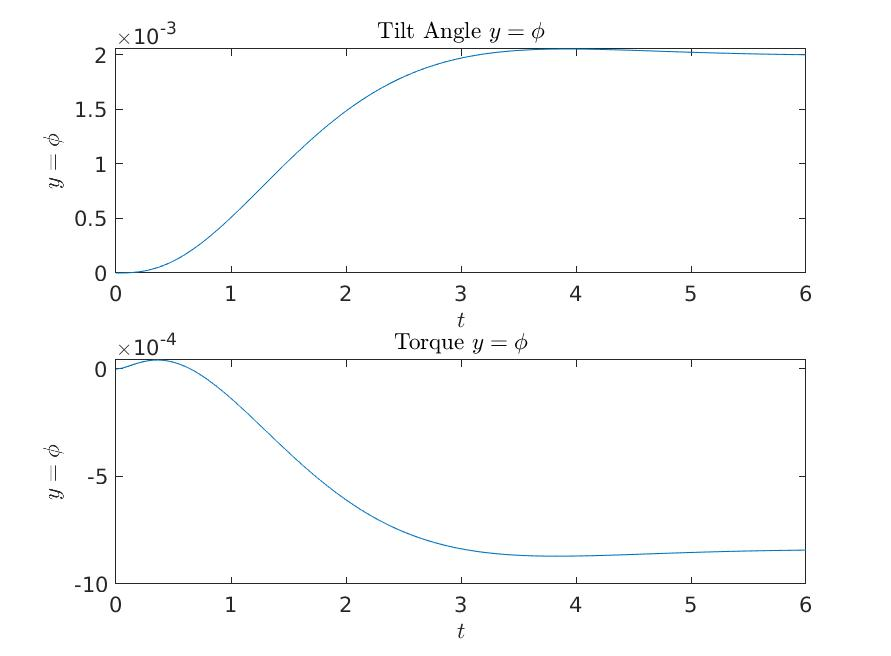
\includegraphics[width = 0.8\textwidth]{ES155P5_2_bicycle.jpg}
            \caption{Steering Angle and Input Torque with step function input using observer feedback}
            \label{fig:HW5_2_c}
        \end{figure}

        \begin{figure}
            \centering
            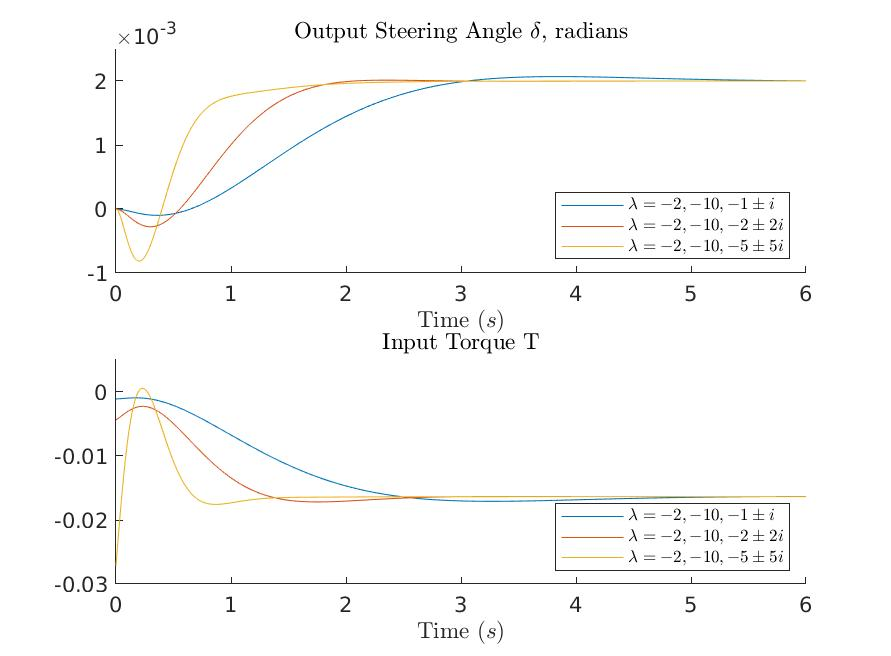
\includegraphics[width = 0.8\textwidth]{../P4/ES155P4_2_bicycleStepResponse.jpg}
            \caption{Steering Angle and Input Torque with step function input with no observer feedback.  Only consider the blue line.}
            \label{fig:HW4_2_c}
        \end{figure}

        


    \end{enumerate}

\end{enumerate}
\end{document}


